%% Beispiel-Präsentation mit LaTeX Beamer im KIT-Design
%% entsprechend den Gestaltungsrichtlinien vom 1. August 2020
%%
%% Siehe https://sdqweb.ipd.kit.edu/wiki/Dokumentvorlagen

%% Beispiel-Präsentation
\documentclass[en]{sdqbeamer} 

%% Footnote without numbering
\newcommand\nonumberfootnote[1]{%
  \begingroup
  \renewcommand\thefootnote{}\footnote{#1}%
  \addtocounter{footnote}{-1}%
  \endgroup
}
 
%% Titelbild
\titleimage{banner_2020_kit}

%% Gruppenlogo
\grouplogo{} 

%% Gruppenname und Breite (Standard: 50 mm)
\groupname{Institute for Automation and Applied Informatics (IAI)}
\groupnamewidth{60mm}

% Beginn der Präsentation

\title[ABAC for Substations]{Certificateless Attribute-Based Server-Aided Cryptosystem\\for Substation Automation Systems (CASC-SAS)}
\subtitle{Master's Thesis Presentation} 
\author[Moritz Gstuer]{Moritz Gstuer}

\date[12.\,02.\,2025]{12. February 2025}

% Literatur
\usepackage[citestyle=authoryear,bibstyle=numeric,hyperref,maxcitenames=2,backend=biber]{biblatex}
\addbibresource{../bibliography/masterthesis.bib}
\bibhang1em

\begin{document}
 
%Titelseite
\KITtitleframe

%Inhaltsverzeichnis
%\begin{frame}{Agenda}
%\tableofcontents
%\end{frame}

\section{Motivation}
\begin{frame}{Motivation}
    \begin{columns}
        \column{.55\textwidth}
        \centering
        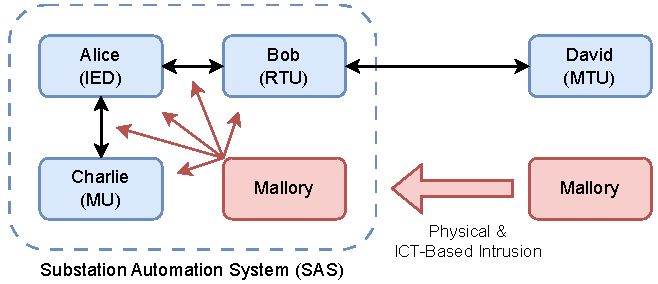
\includegraphics[width=1.0\textwidth]{./figures/sas_intrusion.drawio.pdf}
        \column{.45\textwidth}
        \begin{redblock}{Adversarial Attacks}
            \begin{itemize}
                \item \textbf{Availability-Focused:} Denial-of-Service\\$\rightarrow$ Malware, Flooding, \& Time-Delay
                \item \textbf{Integrity-Focused:} False Data Injection\\$\rightarrow$ Message Forgery, Modification, \& Replay
                \item \textbf{Authenticity-Focused:} Masquerading\\$\rightarrow$ Adaptive Chosen-Message, \& Collusion
            \end{itemize}
            % $\rightarrow$ Authentication, Authorization, Access Control, \& Encryption of Substation Communication
        \end{redblock}
    \end{columns}
    \nonumberfootnote{IED\dots Intelligent Electronic Device | MU\dots Merging Unit | RTU\dots Remote Terminal Unit}
    \nonumberfootnote{MTU\dots Master Terminal Unit | ICT\dots Information and Communications Technology}
\end{frame}
\begin{frame}{Substation Communication}
    \begin{blueblock}{Requirements}
        \begin{itemize}
            \item Integrity
            \item Authenticity
            \item Non-Repudiation
            \item Least Privilege Principle
            \item Separation of Duties
        \end{itemize}
        $\rightarrow$ Authentication, Authorization, \& Access Control
    \end{blueblock}
    \begin{grayblock}{Constraints: IEC 61850 Message Types \& Performance Classes \parencite*{IEC61850P5,IEC61850P8}}
        Client-Server (Unicast) \& Publisher-Subscriber (Broadcast/Multicast) \\$\rightarrow$ Resource \& Time Constraints!
        \\Examples: GOOSE (Type 1A, 3 ms), SV (Type 4, 3 ms), MMS (Type 2/3/5, 100-10000 ms)
    \end{grayblock}
\end{frame}
\begin{frame}{Research Questions}
    \begin{greenblock}{Authorization \& Access Control in SAS}
        How can expressive and flexible yet computationally expensive access control be employed in a SAS?
        \\$\rightarrow$ Policy Evaluation \& Enforcement Strategies
    \end{greenblock}

    \begin{greenblock}{Public-Key Cryptography in SAS}
        How can a secure and lightweight public-key approach be designed, implemented, \& employed in a SAS?
        \\$\rightarrow$ (Dis-)Advantages, \& Speedup Solutions
    \end{greenblock}

    \begin{greenblock}{Security Architecture for Time-Critical Communication}
        How can authentication, authorization, and access control be integrated into a malleable, scalable, and lightweight cryptosystem for time-critical SAS communication?
        \\$\rightarrow$ System Model, Domain Requirements, Architecture, \& Protocols
    \end{greenblock}
\end{frame}

\section{Fundamentals}
\begin{frame}{Attribute-Based Access Control (ABAC)}
    \begin{greenblock}{Definition \parencite{JTF2020}}
        Access control model enabling access decisions based on attributes associated with \textbf{subjects}, \textbf{objects}, \textbf{actions}, and the \textbf{environment} of a system.
    \end{greenblock}
    \begin{blueblock}{Discussion \parencite{Hu2014}}
        \begin{itemize}
            \item Multifactor Policy Expression $\rightarrow$ Fine-Grained \& Flexible Access Control (cf. RBAC/IBAC)
            \item Dynamic Policy Evaluation $\rightarrow$ Dynamic Authorization \& Real-Time Attributes
        \end{itemize}
    \end{blueblock}
\end{frame}
\begin{frame}{Public-Key Cryptography in SAS}
    \begin{blueblock}{Key Distribution \& Identity Verification}
        Unsecure Network \& Untrusted Network Participants
        \\$\rightarrow$ Asymmetric: Lightweight \& Secure Key Distribution
    \end{blueblock}
    \begin{blueblock}{Computational Complexity \parencite{Elbez2019,Ishchenko2018}}
        Example: 1024-Bit RSA Digital Signature vs. 128-Bit HMAC/GMAC
        \\$\rightarrow$ 10 ms vs. 50 µs on RPi2 (1 GHz quad-core)
        \\$\rightarrow$ 0.3 ms vs. 4 µs on Xeon X3440 (2.53 GHz quad-core) 
    \end{blueblock}
\end{frame}

\section{Related Work}
\begin{frame}{Related Work}
    \begin{blueblock}{IEC 62351 \parencite*{IEC62351P6,IEC62351P8}}
        Standard for Cybersecurity: Energy-Related Systems \& Communication Networks
        \\$\rightarrow$ Authenticity \& Integrity: Mandatory Symmetric Authentication
        \\$\rightarrow$ Confidentiality: Optional (Non-Recommended) Symmetric Encryption
        \\$\rightarrow$ Access Control: Role-Based Access Control (RBAC) (Access-Token-Driven, 7 Mandatory Roles)
    \end{blueblock}
\end{frame}
\begin{frame}{Related Work}
    \begin{blueblock}{Secure Communication in Substations}
        \begin{itemize}
            \item Bump-in-the-Wire Security Filter for GOOSE/SV MAC Tagging \& Verification \parencite{Ishchenko2018}
            \item Domain-Based Collaborative Cyberattack Mitigation Approach \parencite{Hong2019}
            \item Fixed-Latency Hardware Architecture for GOOSE/SV Encryption \& Authentication \parencite{Rodriguez2021}
        \end{itemize}
    \end{blueblock}

    \begin{blueblock}{Access Control in Substations}
        \begin{itemize}
            \item XACML-Based RBAC Approach for IEC 61850 \& IEC 62351 compliant SAS \parencite{Lee2015}
            \item Distributed RBAC for Subscription-Based Remote Network Services \parencite{Ma2006} % Constraint-Enabled 
            \item Rule-Based RBAC Policy Enforcement Architecture \parencite{Alcaraz2016} % for Smart Grid Systems
            \item Firewall for ABAC in Smart Grids \parencite{Ruland2018}
            \item ABAC for Real-Time Availability in Highly Dynamic Systems \parencite{Burmester2013}
        \end{itemize}
    \end{blueblock}
\end{frame}
% \begin{frame}{Related Work}
% \begin{table}
%     \centering
%     \begin{tabular}{c c}
%     \toprule
%     %Adversarial Attack & \multicolumn{2}{c |}{Classification} & \multicolumn{5}{c}{Policy}\\
%     %\midrule
%     % Secure Communication in Substations
%     \parencite{Ishchenko2018} & Bump-in-the-Wire Security Filter for GOOSE/SV MAC Tagging \& Verification\\
%     \parencite{Hong2019} & Domain-Based Collaborative Cyberattack Mitigation Approach\\
%     \parencite{Rodriguez2021} & Fixed-Latency Hardware Architecture for GOOSE/SV Encryption \& Authentication\\
%     % Role-Based Access Control (RBAC) in Substations
%     \parencite{Ma2006} & Distributed RBAC for Subscription-Based Remote Network Services\\% Constraint-Enabled
%     \parencite{Lee2015} & XACML-Based RBAC Approach for IEC 61850 \& IEC 62351 compliant SAS\\
%     \parencite{Alcaraz2016} & Rule-Based RBAC Policy Enforcement Architecture\\% for Smart Grid Systems
%     %Attribute-Based Access Control (ABAC) in Substations
%     \parencite{Burmester2013} & T-ABAC: An attribute-based access control model for real-time availability in highly dynamic systems\\
%     \parencite{Ruland2018} & Firewall for Attribute-Based Access Control in Smart Grids\\
%     \bottomrule
%     \end{tabular}
% \end{table}
% \end{frame}

\section{Approach}
\begin{frame}{CASC-SAS Approach}
    \begin{greenblock}{\textbf{C}ertificateless \textbf{A}ttribute-Based \textbf{S}erver-Aided \textbf{C}ryptosystem for \textbf{S}ubstation \textbf{A}utomation \textbf{S}ystems (CASC-SAS)}
        \textbf{Objective:} Fine-grained \& flexible access control relying on dynamic authorization \& authentication
        \\\textbf{Central Concepts:}
        \begin{itemize}
            \item Authentication $\rightarrow$ CASA
            \item Authorization \& Access Control $\rightarrow$ SABAAC
        \end{itemize}
    \end{greenblock}
\end{frame}
\begin{frame}{CASA: Authentication}
    \begin{greenblock}{\textbf{C}ertificateless \textbf{A}ttribute-Based \textbf{S}erver-Aided \textbf{A}uthentication (CASA)}
        Lightweight \& scalable algorithm-agnostic data frame authentication approach
        \\\textbf{Additionally:} $S_{CASA}$ $\rightarrow$ Certificateless attribute-based server-aided signature scheme
    \end{greenblock}
    \begin{blueblock}{Protocol: Algorithm-Agnostic PKC Exchange}
        \textbf{Tasks:} Registration, revocation, query, \& computation
        \\\textbf{Central Component:} CASA Administration and Processing Platform (CAPP)
    \end{blueblock}
    \nonumberfootnote{PKC\dots Public Key Cryptography}
\end{frame}
\begin{frame}{SABAAC: Authorization \& Access Control}
    \begin{greenblock}{\textbf{S}erver-Aided \textbf{A}ttribute-\textbf{B}ased \textbf{A}uthorization \& \textbf{A}ccess \textbf{C}ontrol (SABAAC)}
        Delegation of access policy evaluation to semi-trusted server (PDP)
        \\$\rightarrow$ Enforcement of access control decisions via bump-in-the-wire device (PEP)
    \end{greenblock}
    \begin{blueblock}{Protocol: Delegated Attribute-Based Authorization}
        \textbf{Task:} Creation, modification, storage, and distribution of access control policies
        \\\textbf{Central Components:} PAP \& PDP
    \end{blueblock}
    \begin{blueblock}{Protocol: Delegated Attribute-Based Access Control}
        \textbf{Task:} Request, exchange, \& enforcement of access control decisions
        \\\textbf{Central Components:} PDP \& PEP
    \end{blueblock}
    \nonumberfootnote{PAP\dots Policy Administration Point | PDP\dots Policy Decision Point | PEP\dots Policy Enforcement Point}
\end{frame}
\begin{frame}{Delegated Access Control: Session Initialization}
    \centering
    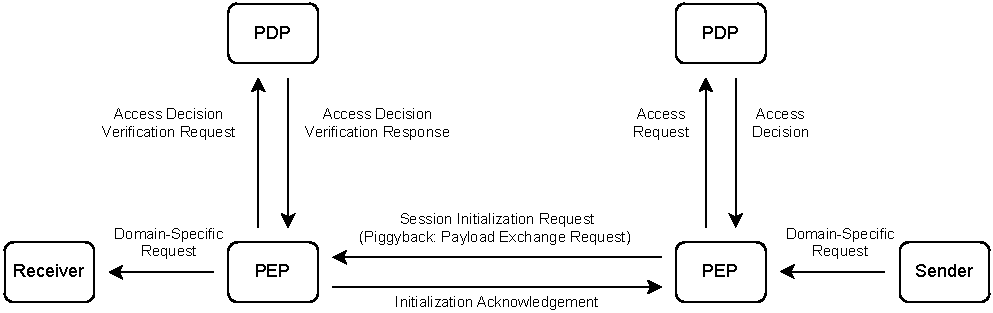
\includegraphics[width=1.0\textwidth]{./figures/SABAAC_protocols_accesscontrol_initialization_shortened.drawio.pdf}
\end{frame}
\begin{frame}{Delegated Access Control: Payload Exchange}
    \centering
    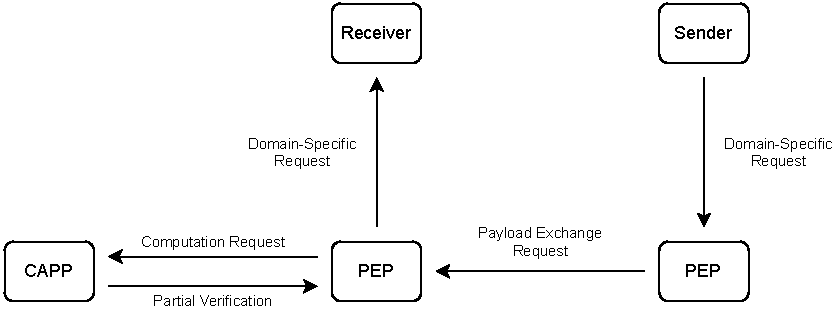
\includegraphics[width=1.0\textwidth]{./figures/SABAAC_protocols_accesscontrol_payloadexchange.drawio.pdf}
\end{frame}
\begin{frame}{CASC-SAS Architecture: Function-Oriented}
    \centering
    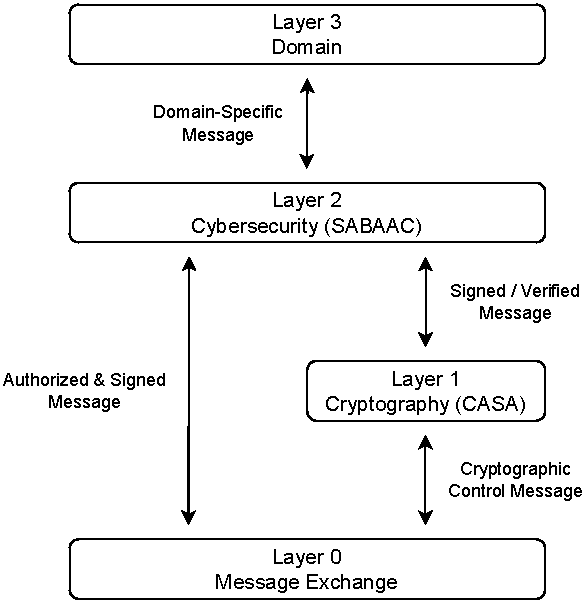
\includegraphics[height=0.75\textheight]{./figures/layers_request_example_shortened.drawio.pdf}
\end{frame}
\begin{frame}{CASC-SAS Architecture: Component-Oriented}
    \begin{columns}
        \column{.65\textwidth}
        \centering
        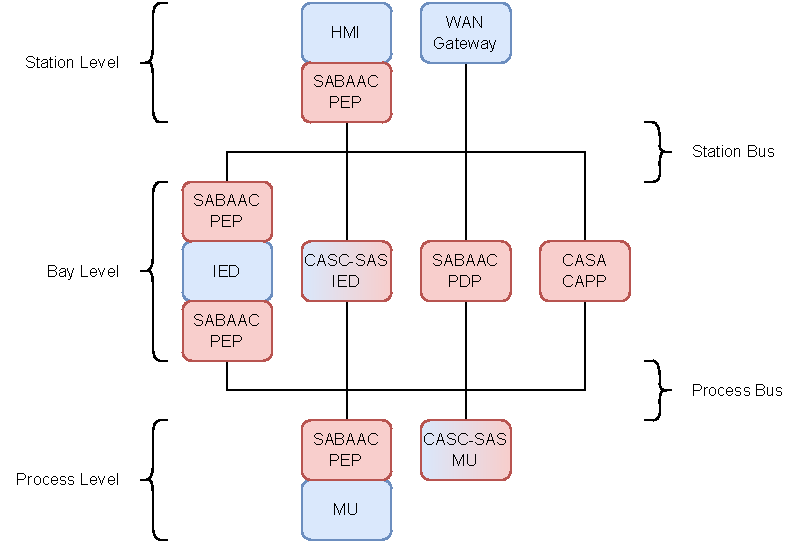
\includegraphics[height=0.75\textheight]{./figures/casc_architecture_color_shortened.drawio.pdf}
        \column{.35\textwidth}
        \footnotesize
        CAPP\dots CASA Administration\\\qquad\qquad\& Processing Platform\\HMI\dots Human-Machine Interface\\IED\dots Intelligent Electronic Device\\MU\dots Merging Unit\\PDP\dots Policy Decision Point\\PEP\dots Policy Enforcement Point\\WAN\dots Wide Area Network
    \end{columns}
\end{frame}

\section{Evaluation}
\begin{frame}{Evaluation: Overview}
    \begin{greenblock}{Goal of Approach}
        Protect substations against domain-typical adversaries \& attacks
        \\\textbf{Communication:} Time-constrained \& traffic-intensive
        \\\textbf{Deployment:} Construction \& Retrofitting
    \end{greenblock}
    \begin{blueblock}{Evaluation}
        Theoretically \& experimentally performed evaluation
        \begin{itemize}
            \item Security Analysis $\rightarrow$ Theorems
            \item Performance Analysis $\rightarrow$ Testbed-based experiments
            \item Compatibility Analysis $\rightarrow$ Laboratory-based experiments
        \end{itemize}
    \end{blueblock}
\end{frame}
\begin{frame}{Security Analysis}
    \begin{greenblock}{Central Question}
        Does CASC-SAS provide security against typical SAS adversaries and attacks?
        \\\textbf{Metrics:} Satisfied requirements, assumed adversary, mitigated attacks, \& change of substation attack surface
    \end{greenblock}
    \begin{blueblock}{Theorems}
        Theorems to demonstrate mitigation strategies for six attacks:
        \begin{itemize}
            \item Message Forgery
            \item Message Modification
            \item Message Replay
            \item Time-Delay
            \item Chosen-Message
            \item Collusion
        \end{itemize}
    \end{blueblock}
\end{frame}
\begin{frame}{Performance Analysis I}
    \centering
    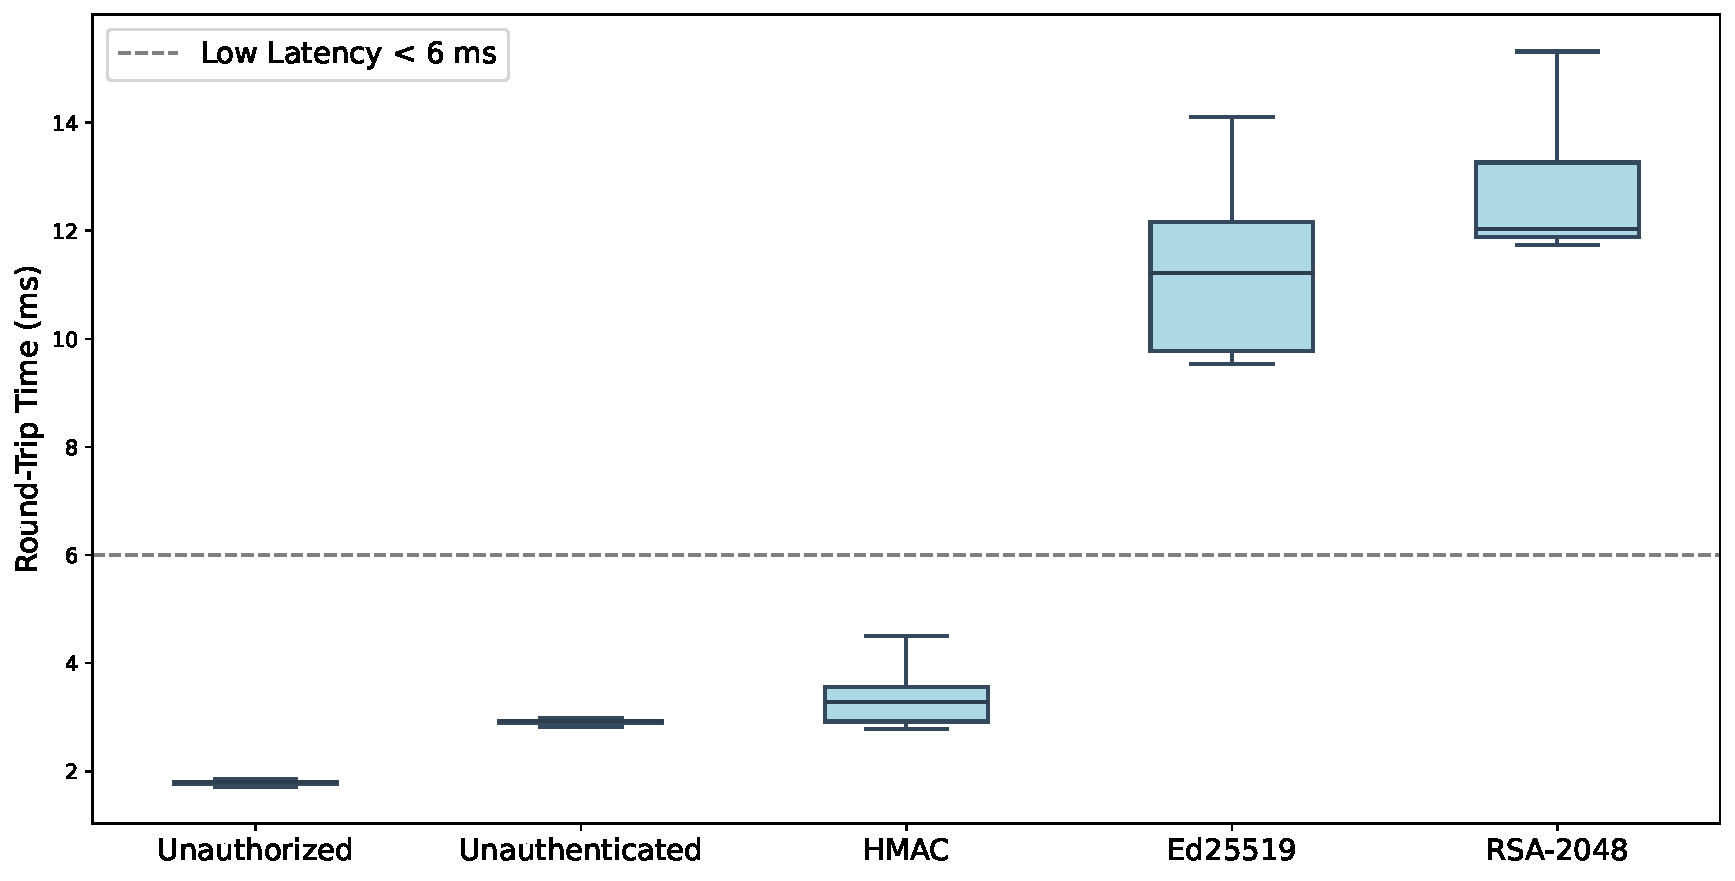
\includegraphics[height=0.75\textheight]{./figures/boxplot_without_casa.pdf}
\end{frame}
\begin{frame}{Performance Analysis II}
    \centering
    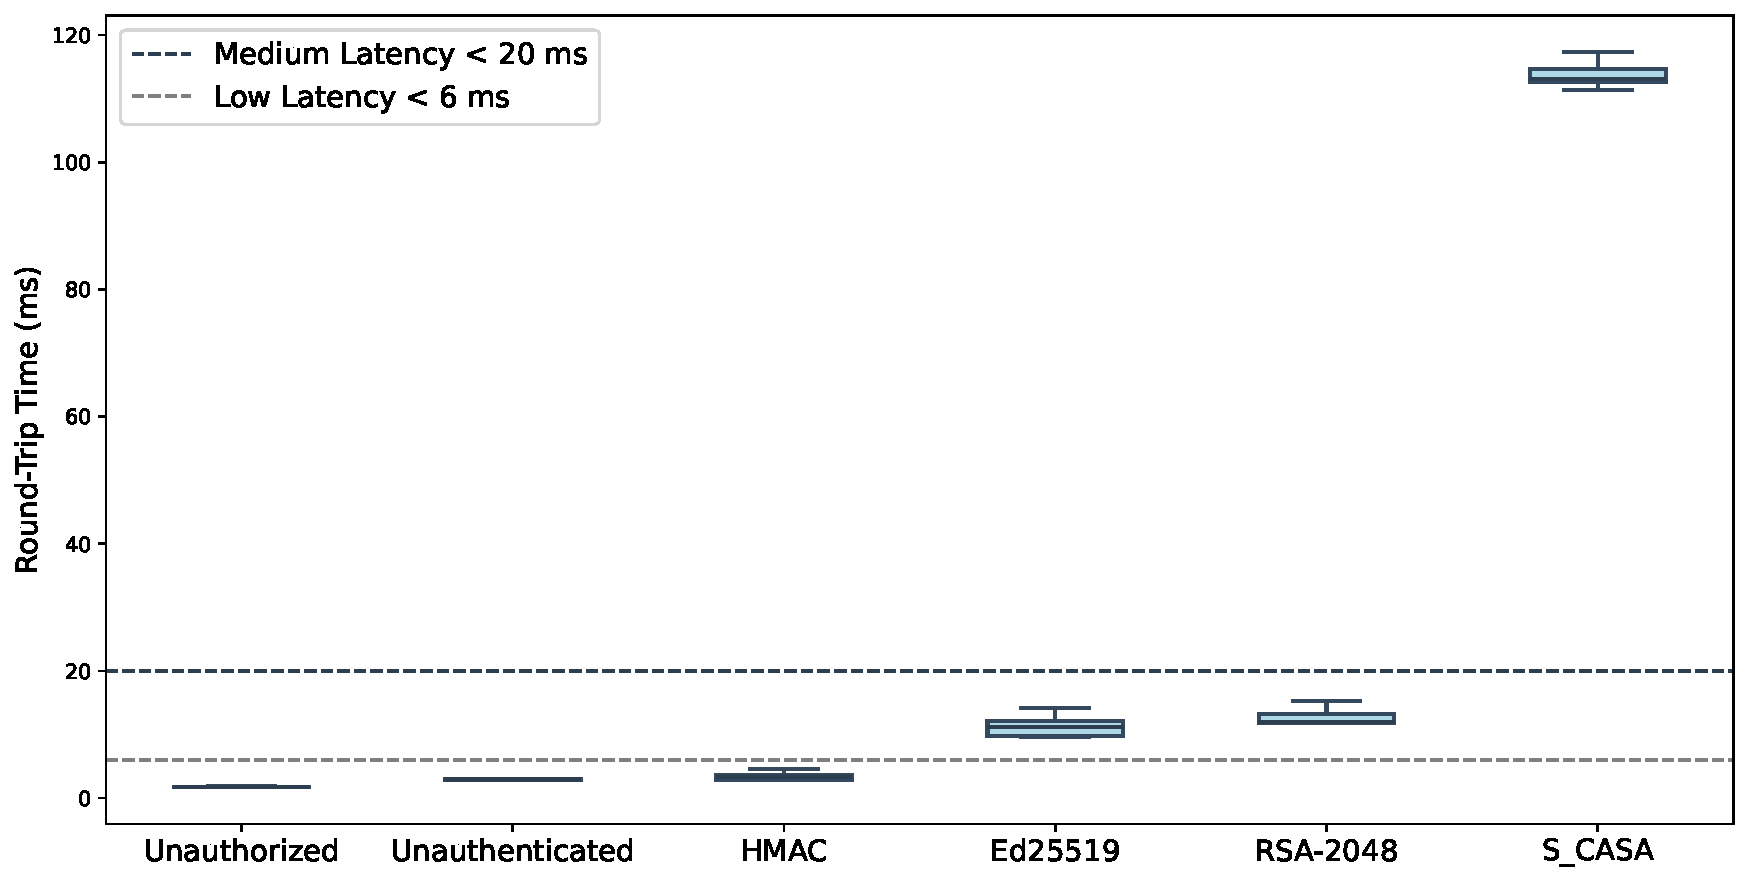
\includegraphics[height=0.75\textheight]{./figures/boxplot_with_casa.pdf}
\end{frame}
\begin{frame}{Compatibility Analysis}
    \centering
    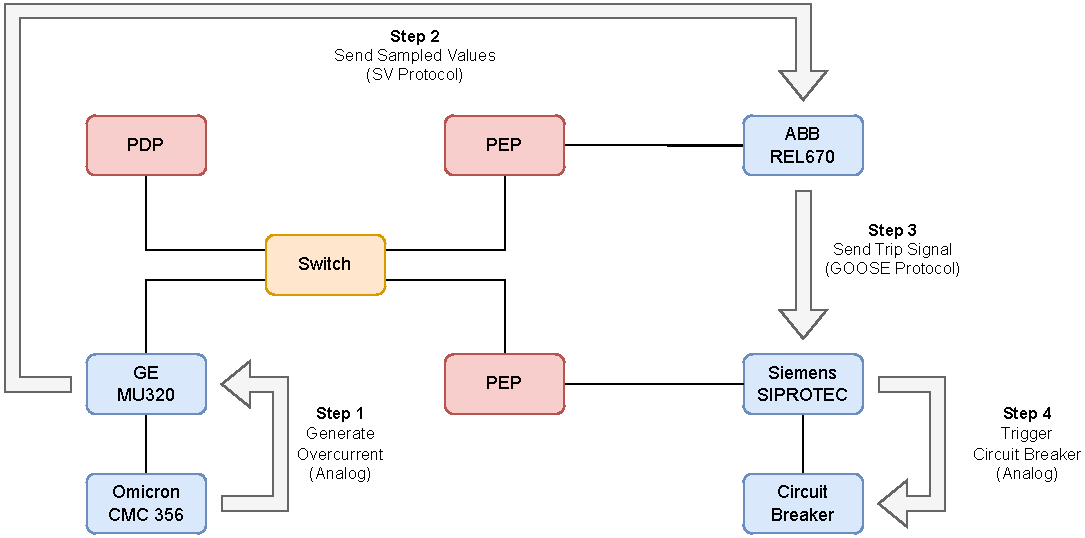
\includegraphics[height=0.75\textheight]{./figures/lab_evaluation_steps_simplified.drawio.pdf}
\end{frame}

\section{Future Work}
\begin{frame}{Future Work I}
    \begin{blueblock}{Cryptography-Driven Authentication, Authorization, \& Access Control}
        Authentication, authorization, \& access control integrated into a single attribute-based PKC scheme
        \\$\rightarrow$ \textbf{Advantage:} Privacy \& Anonymity
    \end{blueblock}
    \begin{blueblock}{Encryption \& Decryption}
        Encryption \& decryption in conjunction with signing \& verification operations
        \\$\rightarrow$ \textbf{Advantage:} Confidentiality
    \end{blueblock}
    \begin{blueblock}{Hardware Acceleration}
        Evaluation of hardware-based cryptography acceleration in a SAS
        \\$\rightarrow$ \textbf{Advantage:} Decreased computation time \& increased message throughput
        \\$\rightarrow$ \textbf{Risk:} Algorithm compatibility, costs per acceleration unit, \& computation time consistency
    \end{blueblock}
\end{frame}
\begin{frame}{Future Work II}
    \begin{blueblock}{AI for Policy Management}
        Integration of CASC-SAS with AI-based intrusion detection for security policy creation \& modification
        \\$\rightarrow$ \textbf{Advantage:} Mitigation of a wider range of cyberattacks in a timelier manner
    \end{blueblock}
    \begin{blueblock}{SDN-Based Realization}
        Aggregation of PEPs by deploying a virtual PEP for each port of a Software-Defined Networking (SDN) switch
        \\$\rightarrow$ \textbf{Advantage:} Reduced costs of deployment \& reduced architectural complexity
    \end{blueblock}
    \begin{blueblock}{Extended Demonstration of Applicability}
        Employment in time-critical systems with similar requirements \& constraints
        \\$\rightarrow$ \textbf{Examples:} Industry 4.0, robotics, avionics, \& medical systems
    \end{blueblock}
\end{frame}

\section{Conclusion}
\begin{frame}{Conclusion}
    \begin{redblock}{Problem}
        Expressive \& flexible access control, \& malleable PKC: Applicable to the SAS domain?
        \\$\rightarrow$ Constrained resources \& communication time
    \end{redblock}
    \begin{blueblock}{Contribution}
        CASC-SAS security architecture \& framework\dots
        \\\dots employs mandatory authentication, authorization, \& access control
        \\\dots for time-critical SAS communication
        \\\dots in time-variable SAS environment.
    \end{blueblock}
    \vspace{0.5em}
    \centering
    \huge
    Thank you!
\end{frame}

\appendix
\beginbackup
\section{System Model}
\begin{frame}{Motivation}
    \begin{columns}
        \column{.4\textwidth}
        \centering
        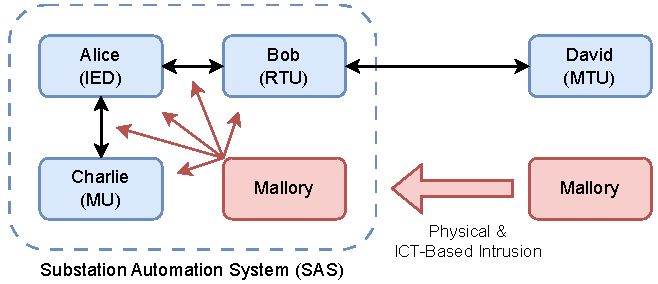
\includegraphics[width=1.0\textwidth]{./figures/sas_intrusion.drawio.pdf}
        \column{.6\textwidth}
        \begin{redblock}{Substation Threats \& Attacks}
            \begin{itemize}
                \item Eavesdropping
                \item Man-in-the-Middle
                \item Spoofing/Masquerading
                \item Replay
                \item Denial of Service\\$\rightarrow$ Flooding, Broadcast/Multicast Storm, \& Poisoning
                \item False Data Injection\\$\rightarrow$ Forged Sensor Data \& Commands, \& Configuration Tampering
            \end{itemize}
            % $\rightarrow$ Authentication, Authorization, Access Control, \& Encryption of Substation Communication
        \end{redblock}
    \end{columns}
\end{frame}
\begin{frame}{System Model: Adversarial Attacks}
    \begin{columns}
        \column{.38\textwidth}
        \centering
        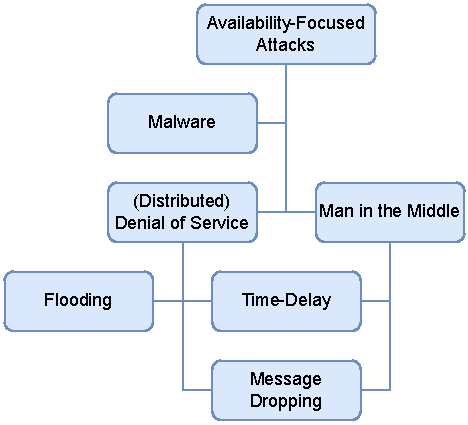
\includegraphics[width=\linewidth]{figures/attacks_availability.drawio.pdf}
        \column{.295\textwidth}
        \centering
        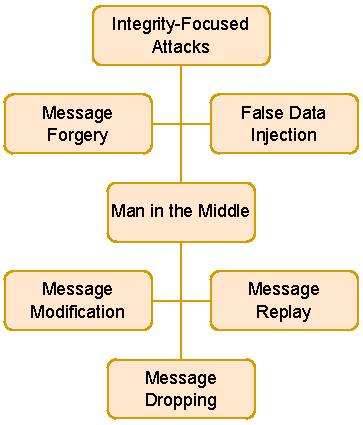
\includegraphics[width=\linewidth]{figures/attacks_integrity.drawio.pdf}
        \column{.30\textwidth}
        \centering
        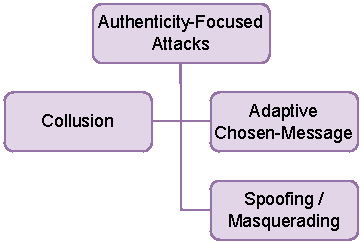
\includegraphics[width=\linewidth]{figures/attacks_authenticity.drawio.pdf}
    \end{columns}
\end{frame}
\begin{frame}{System Model: Substation Automation System (SAS)}
    \centering
    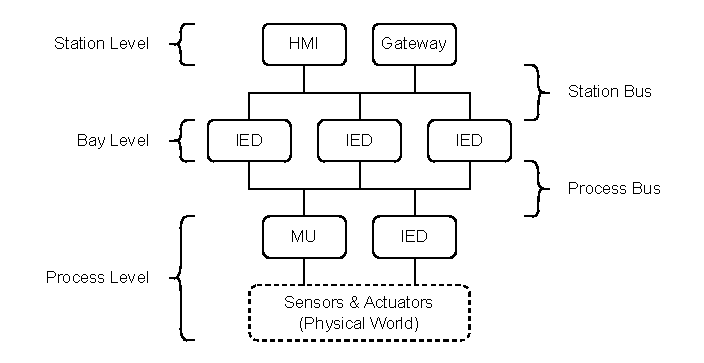
\includegraphics[width=0.7\textwidth]{./figures/substation_architecture.drawio.pdf}
    \nonumberfootnote{IED\dots Intelligent Electronic Device | MU\dots Merging Unit | HMI\dots Human-Machine Interface}
\end{frame}

\section{Fundamentals}
\begin{frame}{Authentication, Authorization, \& Access Control}
    \centering
	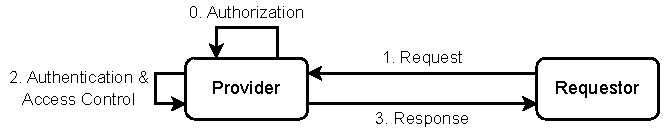
\includegraphics[width=0.9\textwidth]{./figures/access_control_request_traditional.drawio.pdf}
    \begin{redblock}{Problem}
        Too many provider responsibilities
        \\$\rightarrow$ Policy Management/Decisions/Enforcement, Request Verification, \& Response Creation
    \end{redblock}
\end{frame}

\section{Related Work}
\begin{frame}{Related Work}
    \begin{blueblock}{Attribute-Based Access Control (ABAC) in Substations}
        \begin{itemize}
            \item Firewall for Attribute-Based Access Control in Smart Grids \parencite{Ruland2018}
            \\$\rightarrow$ Firewall with XACML-Based ABAC Policies
            \\$\rightarrow$ Outer \& Inner Station Bus
            \\$\rightarrow$ Unobstructed Fast Messages (e.g. GOOSE)
            \item T-ABAC: An attribute-based access control model for real-time availability in highly dynamic systems \parencite{Burmester2013}
            \\$\rightarrow$ Real-Time Attribute Values
            \\$\rightarrow$ Labeling of High Priority Packets
            \\$\rightarrow$ Domain-Based Congestion Avoidance
        \end{itemize}
    \end{blueblock}
    % Message Authentication, Asym. Performance Evaluation, BitW- \& HW-Solutions, Access Control
\end{frame}

\section{Approach}
\begin{frame}{CASC-SAS Architecture: Function-Oriented}
    \centering
    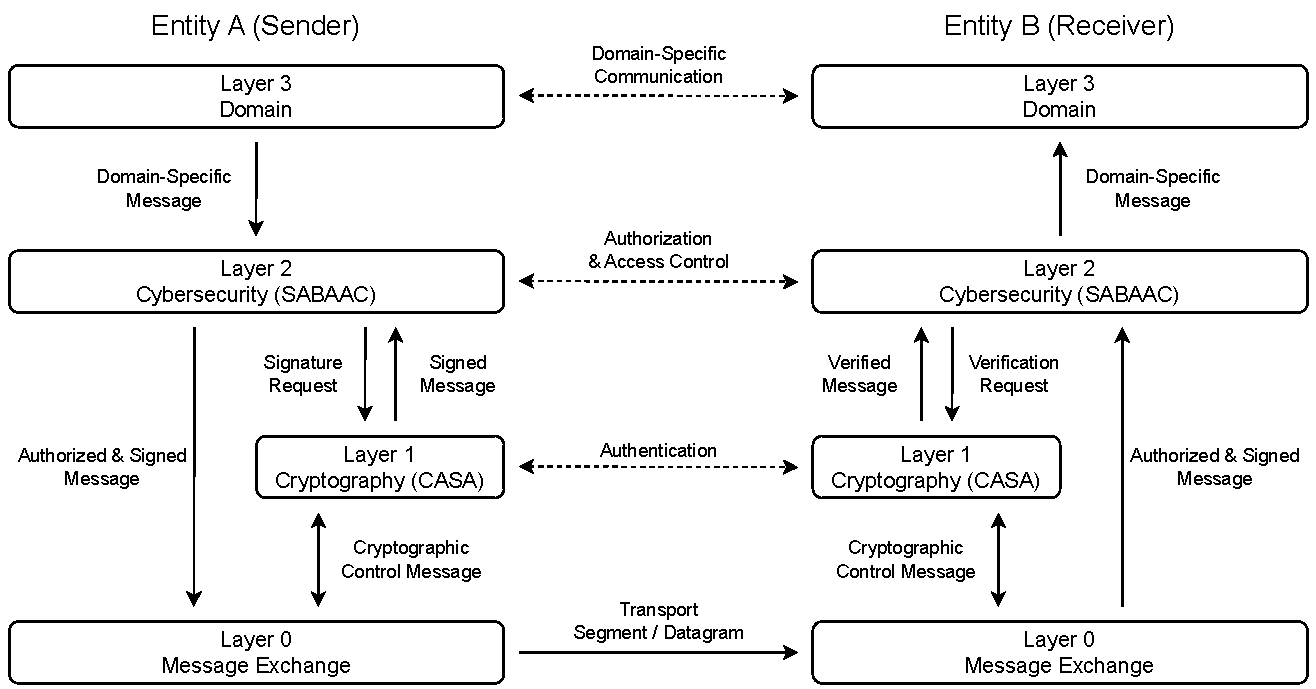
\includegraphics[height=0.75\textheight]{./figures/layers_request_example.drawio.pdf}
\end{frame}
\begin{frame}{CASC-SAS Architecture: Component-Oriented}
    \begin{columns}
        \column{.65\textwidth}
        \centering
        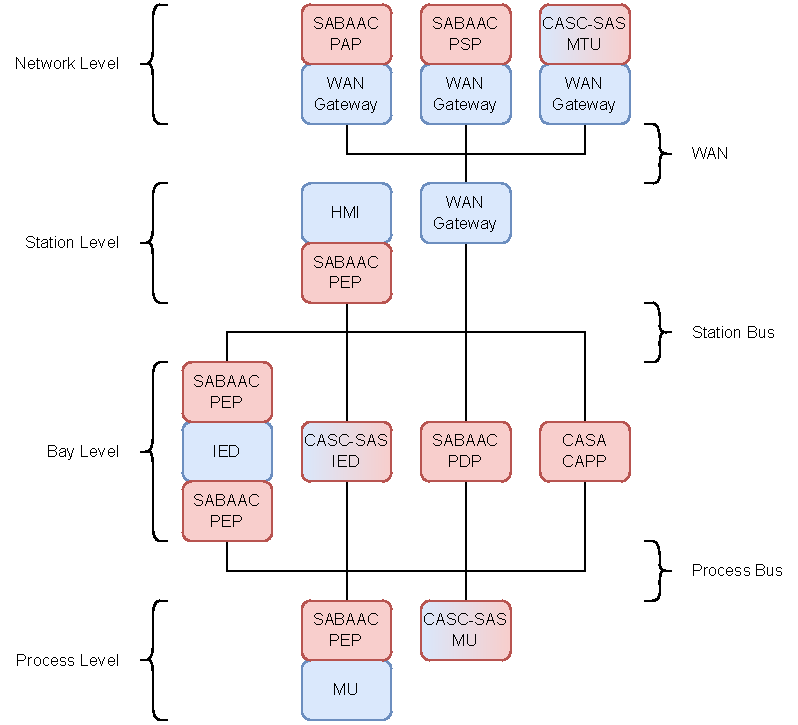
\includegraphics[height=0.75\textheight]{./figures/casc_architecture_color.drawio.pdf}
        \column{.35\textwidth}
        \footnotesize
        CAPP\dots CASA Administration\\\qquad\qquad\& Processing Platform\\HMI\dots Human-Machine Interface\\IED\dots Intelligent Electronic Device\\MTU\dots Master Terminal Unit\\MU\dots Merging Unit\\PAP\dots Policy Administration Point\\PDP\dots Policy Decision Point\\PEP\dots Policy Enforcement Point\\PSP\dots Policy Storage Point\\RTU\dots Remote Terminal Unit\\WAN\dots Wide Area Network
    \end{columns}
\end{frame}

\begin{frame}[allowframebreaks]{References}
\printbibliography
\end{frame}

\backupend

\end{document}